\documentclass{IEEEcsmag}

\usepackage[colorlinks,urlcolor=blue,linkcolor=blue,citecolor=blue]{hyperref}

\usepackage{upmath}
\usepackage{amssymb}
\usepackage{amsmath}
\usepackage{array}
\newcolumntype{P}[1]{>{\centering\arraybackslash}p{#1}}

\jvol{XX}
\jnum{XX}
\paper{8}
\jmonth{May/June}
\jname{Computing in Science and Engineering}
\pubyear{2021}
\newtheorem{theorem}{Theorem}
\newtheorem{lemma}{Lemma}

\setcounter{secnumdepth}{0}

\begin{document}

\sptitle{Department: Head}
\editor{Editor: Name, xxxx@email}

\title{PyExaFMM: Designing a high-performance point fast multipole solver in Python with Numba}

\author{S. Kailasa}
\affil{Department of Mathematics, University College London}

\author{T. Betcke}
\affil{Department of Mathematics, University College London}

\author{T. Wang}
\affil{Department of Mechanical and Aerospace Engineering, The George Washington University}

\author{\text{L}. A. Barba}
\affil{Department of Mechanical and Aerospace Engineering, The George Washington University}

\markboth{Department Head}{Paper title}

\begin{abstract}
The Fast Multipole Method is a good case study for understanding the maturity of Python for developing high-performance software due its reliance on a complex hierarchical tree data structure. In this article we explore the software engineering and mathematical techniques used to extract performance for PyExaFMM, a Python based solver accelerated with Numba. We achieve runtimes within $\mathcal{O}(10)$ of the state of the art C++ implementation, with comparable accuracy, for three dimensional electrostatic problems in single precision.
\end{abstract}

\maketitle
\chapterinitial{We introduce PyExaFMM}\footnote{Available at https://www.github.com/exafmm/pyexafmm} a Python-based solver for the point Fast Multipole Method [FMM], designed for high-performance computing [HPC]. The appeal of developing scientific software in Python lies in the ease of developing prototypes, the ubiquity of Python skills amongst computational scientists, as well as the availability of simple cross platform builds via Conda. The FMM algorithm is non-trivial, relying on the traversal of a hierarchical tree. Therefore it represents a challenge to efficiently represent its operations, and offers a good case-study to examine the maturity of Python for building HPC applications.

PyExaFMM is a single precision, single node, implementation designed for three-dimensional problems. We implement parallel strategies for multicore architectures, similar to \cite{Bramas2020, Wang2021}. As with all Python applications, performance is degraded by portions of code that are unavoidably interpreted. However, this represents a compromise between usability and performance. Using lines-of-code [LOC] as a rough metric of usability, PyExaFMM consists of approximately 5,800 LOC, compared with approximately 20,000 LOC and 50,000 LOC for comparable C++ implementations, ExaFMM-T and TBFMM, respectively \cite{Bramas2020, Wang2021}.

In this article we begin by providing an overview of the FMM algorithm, as well as the Kernel-Independent [KIFMM] variant
\cite{Ying2004} used by PyExaFMM. We proceed to introduce Numba, and discuss how it is used to accelerate computations. We continue by examining other mathematical and software based optimizations used to extract performance. Specifically, the efficient pre-computation, and application of FMM operations, and an overview of the software's design. We conclude with a comparison of performance, in terms of accuracy, runtimes, and memory footprint, with the comparable state-of-the-art [SOTA] C++ implementation from the ExaFMM project, ExaFMM-T \cite{Wang2021}.

\section{FAST MULTIPOLE METHODS}

\subsection{The N-Body Problem}

The FMM \cite{Greengard1987}, approximates the solution of the `$N$ body problem', in which one seeks to calculate pairwise interactions between $N$ objects. This arises in numerous contexts in science and engineering, for example in the calculation of electrostatic potential due to a set of charged particles. Using this problem in three dimensions as our model to explore the FMM, the potential, $\phi(x_j)$, for a given point at position $x_j$, or `target', due to $N$ points at positions $x_i$, or `sources', where $i \in [1, ..., N]$, each with a charge $q_i$, can be written as,

\begin{eqnarray}
	\phi(x_j) = \sum_{i=1}^{N} K(x_i, x_j) q_i,
\label{eq:sec:intro:nbody_problem}
\end{eqnarray}

here $K(\cdot, \cdot)$ is called the Green's function, or kernel function. For our model problem it is,

\begin{eqnarray}
	K(x, y) = \frac{1}{4\epsilon_0\pi|x-y|},
\label{eq:sec:intro:laplace_kernel}
\end{eqnarray}

and is referred to as the Laplace kernel, where $\epsilon_0$ is the permittivity of free space. Without loss of generality, we consider the set of sources and set of targets to correspond to the same set of points. Attempting to evaluate the sum in (\ref{eq:sec:intro:nbody_problem}) directly for $N$ points, results in algorithm of $\mathcal{O}(N^2)$ runtime complexity. However, the FMM is able to approximate (\ref{eq:sec:intro:nbody_problem}) with just $\mathcal{O}(N)$ runtime complexity and proscribed error bounds, making the simulation of physically realistic systems tractable.

\subsection{The FMM Algorithm}\label{sec:intro:algorithm}

The key idea behind the FMM is to encode the potential in the far field due to a cluster of points with a representative analytic series expansion centered on the cluster, known as a \textit{multipole expansion}. This expansion can be truncated to tune for a desired accuracy, allowing one to approximate the sum in (\ref{eq:sec:intro:nbody_problem}). Alternatively, the expansion can be centered away from the cluster, and is then known as a \textit{local expansion}. We can translate the expansion centers of multipole or local expansions without a loss of accuracy, as well as between multipole and local expansion representations of a cluster. This is critical in the development of the $\mathcal{O}(N)$ algorithm. Note, the approximation is only valid where the kernel function of a problem exhibits appropriate `decay' characteristics, allowing us to assume that potential due to clusters of points far away from a region of interest can be well approximated with a truncated representative expansion.

In the FMM, the problem domain is described by a cubic box enclosing all targets and sources, which is hierarchically partitioned into a an \textit{octree} in three dimensions. Partitioning is recursive, initially the domain is partitioned into eight equal parts in three dimensions, known as its children. The unrefined box is referred to as their parent. The children are each subsequently refined in a similar fashion. The final tree consisting of a series of hierarchically nested boxes.

The size of the box is described by its `level', with level 0 denoting the unrefined box, level 1 denoting its children, and so on. One can define the maximum level of refinement through a  constraint dictating the maximum number of points within the finest box covering a subset of the domain. These finest boxes that remain after refinement are known as leaves. Note that the set of all leaves cover the entire domain, without overlap. One can choose to refine \textit{adaptively}, such that the leaves may be of different sizes, reflective of the underlying point distribution, or \textit{non-adaptively}, such that the leaves are all of a uniform size.

The FMM then consists of two sequential traversals of this tree, where boxes are considered level by level. Initially, during the \textit{upward pass}, multipole expansions for points contained in the leaves are formed. This is referred to as the \textit{point-to-multipole} [P2M] step. In order to obtain the multipole expansions for their parents, the expansion centers of a given box's children are shifted to the center of their shared parent box, and their coefficients are summed. This is referred to as the \textit{multipole-to-multipole} [M2M] step. This is repeated bottom-up, starting at the leaf level, considering boxes level by level, until one is left with the multipole expansions of all boxes in the tree.

Subsequently, during the \textit{downward pass}, the multipole expansions of non-adjacent boxes at the same level of a given box (not sharing an edge, face, or corner) are defined as being in its far field. In order to evaluate their contribution towards the potential for points within a given box, one translates their multipole expansion to a local expansion centered at the given box. This is referred to as the \textit{multipole-to-local} [M2L] step. The local expansion is then transferred to the children of the given box by shifting the expansion center to the center of the child boxes, and updating the coefficients of the child boxes' local expansions. This is referred to as \textit{local-to-local} [L2L] step. Proceeding top-down starting at level 2, considering boxes level by level, one is left with the local expansions for each box. The downward pass starts at level 2 as prior levels only contain near field interactions, with no M2L translations.

The extent of the far field not already encapsulated in the local expansion shrinks as we descend down the levels of the tree, as the far field of a box's parent is already captured in the child's local expansion. The local expansion compresses all of the contribution from the far field towards the potential for targets within a given box.

The evaluation of the local expansion at the target points in a given leaf box is known as the \textit{local-to-point} [L2P] step. Finally, the near fields of a given leaf box, composed of adjacent boxes (sharing an edge, face, or corner), are evaluated directly using (\ref{eq:sec:intro:nbody_problem}), this is referred to as the \textit{point-to-point} [P2P] step. As there are a fixed number of points per leaf node, the complexity of this direct evaluation is bounded.

The $\mathcal{O}(N)$ runtime complexity is the result of the analytic translations between the multipole and local expansion for boxes deemed to be in the far field of a given box, as well as the recursive procedure of the FMM. Due to this, each box only considers interactions with a constant number of other boxes. As there are $\mathcal{O}(N)$ boxes in a given tree, the entire algorithm can be seen to be bounded by a runtime complexity of $\mathcal{O}(N)$.

\subsection{The KIFMM Algorithm}

PyExaFMM utilizes the KIFMM \cite{Ying2004}. This algorithm represents the multipole expansions due to a cluster of charges as set of equivalent charge densities supported on a surface enclosing the cluster. The fields generated by the charges are matched with an equivalent field generated by these equivalent densities by matching the potential they generate at another surface in the far field. This method generalizes the FMM to non-oscillatory problems described by second-order elliptic partial differential equations with constant coefficients, for example the Laplace or Stokes equations. This includes many common problems, such as our model electrostatic problem.

Consider the P2M step illustrated in figure (\ref{fig:operators}a). A cubic \textit{equivalent surface}, sharing the same center, $S_e$ is used to enclose a leaf, and its set of points. It is discretized with evenly spaced quadrature points on its faces, each of which supports an equivalent charge density. To find the equivalent densities, we match the potential generated by the points directly, $\phi_c$, calculated using (\ref{eq:sec:intro:nbody_problem}) with that generated by the equivalent densities at the \textit{check surface}, $S_c$, in the far field, also centered on the box, which encloses both the box and the corresponding equivalent surface. Using (\ref{eq:sec:intro:nbody_problem}) we find,

\begin{equation}
	\sum_{x_i \in S_e, x_j \in S_c} K(x_i, x_j)q_i = \phi_c
	\label{eq:sec:intro:kifmm:p2m1}
\end{equation}

where $x_i$ and $x_j$ are the quadrature points for the equivalent and check surfaces respectively, $q_i$ is the equivalent charge density supported at $x_i$. Written in matrix form, we can write the vector of equivalent densities, $q_e$, as the solution of the following linear system,

\begin{flalign}
	K q_e = \phi_c \\
	q_e = K^{-1} \phi_c
	\label{eq:sec:intro:p2m2}
\end{flalign}

where $K$ denotes a matrix with elements,

\begin{equation}
	K_{i, j} = K(x_i, x_j), \> \> \> x_j \in S_c, \> \> x_i \in S_e
	\label{eq:sec:intro:kifmm:matrixelements}
\end{equation}

We identify these equivalent densities as a multipole expansion. The order of this expansion, $p$, is related to the number of the quadrature points, $n$, by,

\begin{equation}
	n = 6(p-1)^2+2
	\label{eq:sec:intro:kifmm:nquads}
\end{equation}

Equation (\ref{eq:sec:intro:p2m2}) is in general ill-conditioned, therefore we use a truncated singular value decomposition [SVD] of $K$, to calculate a pseudo-inverse. Cutting off components corresponding to singular values smaller than machine epsilon in single precision.

As shown in figure (\ref{fig:operators}a), the equivalent surface is enclosed by the check surface for the P2M step. When this is the case we refer to the surfaces as the \textit{upward} equivalent and check surface respectively. We find that setting the ratio of the side-length of the upward equivalent and check surfaces with respect to the tree node as 1.05 and 1.90 work well in practice.

We perform a similar calculation for the M2M step, illustrated in figure (\ref{fig:operators}b). Here the upward equivalent density of a child box, is matched to that of its parent,

\begin{equation}
	K_c q_e^{child} = K_p q_e ^{parent}
\end{equation}

where $K_c$ and $K_p$ are matrices with elements as defined by (\ref{eq:sec:intro:kifmm:matrixelements}), where $S_c$ and $S_e$ denote their relevant check and equivalent surfaces. To find the child's contribution to the parent's upward equivalent density, and hence multipole expansion, we solve,

\begin{equation}
	q_e^{parent} = K_p^{-1}K_c q_e^{child}
\end{equation}

we refer to $K_p^{-1}K_c$ as the \textit{M2M operator}, with eight unique operators in three dimensions corresponding to all the children of a given box. To find the corresponding \textit{L2L operators} and \textit{M2L operators}, we simply repeat the procedure with the appropriate check and equivalent surfaces. For the L2L step, the check surface is placed inside the equivalent surface. This reflects the region in which we expect the local expansion to valid. Here the surfaces are referred to as the \textit{downward} check and equivalent surfaces respectively. For the M2L step (fig. \ref{fig:operators}d) the potential generated by the upward equivalent densities of the source box, is matched to the that generated by the downward equivalent densities of the target box.

We choose the upward equivalent surface to correspond to the downward check surface, and the downward equivalent surface to correspond to the upward check surface, for a given level. We then notice that the quantity $K^{-1}$ in (\ref{eq:sec:intro:p2m2}) can be re-used in the calculation of the M2M operator, as well as the M2L operator. Additionally, the M2M and L2L operators remain constant for all levels in the tree.

% Larger figure
\begin{figure*}
	\centerline{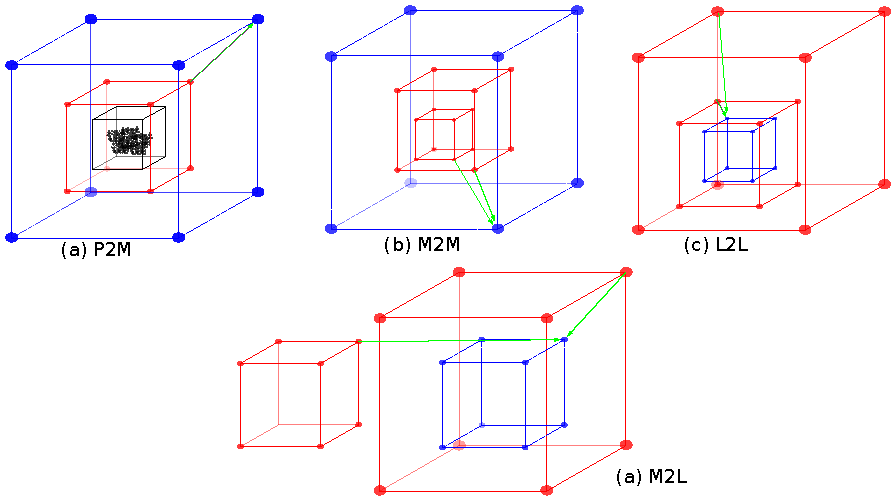
\includegraphics {figures/operators.pdf}}
	\caption{The operators of the KIFMM. Equivalent surfaces are shown in red, check surfaces in blue, and the charged points in black. Surfaces are plotted with 8 quadrature points, one at each vertex.}
	\label{fig:operators}
\end{figure*}

PyExaFMM uses adaptive octrees, for which there are further permutations in the composition of the near and far field. Consider a leaf target box $T$, all source boxes $S$ adjacent to $T$ (sharing an edge, face, or corner) are in $T$'s \textit{U list}. Denoting an adjacent box at the same level as a \textit{colleague}. The children of $T$'s colleagues which are not adjacent to $T$ are in its \textit{W list}, and the children of the colleagues of $T$'s parent which are not adjacent to $T$ are in its \textit{V list}. Finally, the \textit{X list} consists of boxes for which $T$ is in their W list. The X and W list are only calculated for leaf boxes. Collectively these lists are known as the \textit{interaction lists} of $T$.

Greater specification of the interaction lists allows for a more efficient algorithm implementation. Considering a source box in $T$'s W list, the multipole expansion of the source box is valid despite note being in $T$'s far field, therefore reducing the cost of calculating the near field contribution. This is known as a \textit{multipole-to-point} [M2P] operation. For source boxes in $T$'s X list, the multipole expansion is not valid, as $T$ is not in the far-field of the source box. However, the source charges can be evaluated directly at the quadrature points on $T$'s downward equivalent surface. This is known as a \textit{source-to-local} [S2L] operation.

PyExaFMM also enforces a \textit{2:1 balance constraint} on the leaves, such that neighboring leaves may at most differ by one level. This constraint ensures small interaction lists, in the case of highly non-uniform point distributions.

Implementing performant KIFMMs relies on efficiently caching and loading the matrices used in the P2M, M2M, L2L and M2L steps. As the algorithm consists of a series of matrix-vector products, one has to find a way to represent the coefficients of the multipole and local expansions, as well as tree nodes, to take advantage of the cache-locality and vectorization offered by modern processors. The P2P, P2M and M2L steps are the largest bottlenecks in implementing fast KIFMMs \cite{Lashuk2012}. The M2L step has to be applied to each box in a given target box's V list, which is up to 189 times in three dimensions. The P2M step involves calculating the potential due to all points in all leaves at their check surfaces, and the P2P step involves calculating near field interactions directly for all leaves. However, the P2M and P2P steps are embarrassingly parallel over leaves, as is the M2L step over a given V list.

\section{HIGH PERFORMANCE PYTHON WITH NUMBA}

Numba is a just-in-time [JIT] compiler for operating on ndarrays, the multi-dimensional array objects provided by Numpy. Ndarrays have become the basis for numerical computing in Python as Numpy binds to widely used HPC libraries written in C or Fortran, such as LAPACK and BLAS. Numba bypasses the Python interpreter by translating array operations into efficient architecture dependent machine code.

Numba extends Numpy by removing inefficient layers of indirection for indexing into Numpy arrays, instead translating array index operations into direct load and store operations from pointers \cite{Lam2015}. It offers simple multithreading support through a `prange' statement that allows one to loop over processes, mirroring OpenMP's parallel for loops. Numba even supports automatic single-instruction-multiple-data [SIMD] vectorization. Adapting to the instruction set architecture of your CPU, whether it supports Advanced Vector Extensions [AVX], AVX-512, or  Streaming SIMD Extensions [SSE]. Therefore with Numba it is easy to optimize methods that loop over arrays. Furthermore, Numba allows one to decorate functions to be run on GPUs, allowing the development of heterogenous applications with a single Python source.

Importantly, Numba is designed to be a `drop-in' tool, installed simply via a package-manager, with objects marked to be optimized with a decorator. If it is unable to perform an optimization, it fails silently, deferring to the ordinary Python runtime. Therefore developers are able to seamlessly incorporate Numba into new or existing projects. Previously, achieving similar behavior in Python would have required the usage of a hybrid language such as Cython, or by writing custom C extensions on top of CPython.

Numba has been extended with optimized versions of many common array operations, as well as common linear algebra routines available through the Numpy library, such as matrix multiplication. These are called automatically when used in a marked object. For array operations, Numba is able to achieve comparable performance with compiled languages. Consider the evaluation of (\ref{eq:sec:intro:laplace_kernel}) over 100,000 randomly distributed source and target points, where coordinate values, and source charge densities are chosen in interval $[0, 1)$. A Numba modified PyExaFMM takes $4.71 \pm 0.29$ s compared to $1.99 \pm 0.01$ s ExaFMM-T's C++ implementation, where measurements are repeated seven times for statistics \footnote[2]{Note that all benchmarks are reported on a six core Intel i7-9750H CPU.}, and both implementations are SIMD vectorized.

\section{TECHNIQUES FOR ACHIEVING PERFORMANCE}

\subsection{Tree Construction}

Box positions in the tree are encoded in a 64-bit \textit{Morton key} \cite{Sundar2007}. A box at a given level, $l$, has an integer displacement along a given axis in the range $[0, 2^l)$, which we call an index. In three dimensions, the bits of these indices are interleaved as,

\begin{equation}
	\label{eq:morton_encoding}
	x_1y_1z_1...x_ny_nz_n | l,
\end{equation}

where $x_i$ is the $i^{th}$ bit of the $x$ index, and the level is appended to the tail. We can find the parent of a given key by removing the trailing three index bits. Noticing that the displacement of indices for a given axis is consistent in (\ref{eq:morton_encoding}), we optimize Morton encoding by storing the correctly displaced indices for each axis, up to values of $2^8$, in a lookup table. We then consider 8 bits at at time of each index along a given axis, using only simple bitwise instructions to construct the encoding. Numba is used to optimize a loop through a two dimensional array containing a set of indices along each axis for all boxes being encoded.

The strategy of representing operations in terms of simple instructions and optimizing their application via Numba over a loop of an array, is repeated throughout PyExaFMM. As Numba is most efficiently able to translate basic instructions, with as little use of the Python object model as possible, as well as operations over Numpy arrays. Numba decoration has a marked impact on the performance of common methods used in Morton encoding. For example, finding the adjacent keys of a given Morton key, $1.041 \pm 0.003$ $\mu$s vs  $63 \pm 1$ $\mu$s, finding its parent $171 \pm 1$ ns vs $573 \pm 3$ ns, encoding a point's physical coordinates $685 \pm 19$ ns vs $6.170 \pm 0.001$ $\mu$s and decoding a key into its indices $381 \pm 7$ ns vs $16.500 \pm 0.002$ $\mu$s. \footnote[3]{Note that all statistics are taken with respect to 7 runs, errors corresponding to the standard deviation of results reported to 1 significant figure unless otherwise specified.}

To find a linear representation of the tree representing a set of points, we calculate Morton keys for each point at level 1 which are then stored as a vector. This is repeated top-down, level by level, considering batches of points sharing the same key and refining boxes until the maximum points-per-leaf constraint is met, leaving us with a set of leaves. Where we implement multithreading over batches sharing a key. To `complete' the tree from a linear representation of its leaves, we find their ancestors by repeatedly applying the parent finding function to a leaf. Balancing is then achieved by considering all keys level by level, bottom-up. A given key's parent, and its parent's neighbors are added to the tree if not already present. Overlaps are removed from this final collection, favoring the finest box that covers a given area. This enforces a 2:1 balance. Numba offers optimized implementations of many Python datatypes. Therefore, we are able to represent this algorithm naturally using operations on sets. These implementations are built on top of ndarrays, so we are able to easily convert to a linear array representation of the balanced leaves and their corresponding complete tree.

We can traverse the tree via index lookups, for example to find the parent or neighbors of a given key. These indices are precomputed and stored in a typed Numba dictionary. The coefficients of the multipole and local expansions, as well as the target potentials, for all boxes are each stored in a single vector, which are aligned using the index lookup dictionaries. This scheme is designed for maximum cache-reuse.
Building and balancing a tree with 1,000,000 randomly distributed points, setting the maximum points-per-leaf constraint at 150, takes $2.75 \pm 0.04$ s in PyExaFMM in comparison to $0.64 \pm 0.01$ s with ExaFMM-T.

\subsection{Efficient Operators}

Matrices for the unique M2M and L2L operators, as well that used in the P2M operation, are precomputed and cached in a HDF5 database, and are loaded into memory at runtime.

The M2L operator is handled differently. We notice that there are at most $7^3-3^3=316$ unique M2L operators for a given level in three dimensions corresponding to source and target box pairs, these are described uniquely with a \textit{transfer vector} between a source and target \cite{Fong2009}. We can concatenate them in a single matrix representing the M2L matrices for a given level,

\begin{equation}
    K_{M2L}^{l} = \left [ K^l_1 | K^l_2 | ... | K^l_{316} \right],
    \label{eq:2_4_concatenated_m2l}
\end{equation}

where $K_{M2L}^l \in \mathbb{R}^{m \times 316n}$ is the concatenated M2L matrix, and $K_i^l \in \mathbb{R}^{m \times n}$ is the $i^{th}$ M2L matrix, at level $l$, where there the check and equivalent surfaces are discretized with $m$ and $n$ quadrature points respectively.

We find a compressed representation using the randomized SVD of Halko et. al \cite{Halko2011}. We introduce this algorithm following the discussion in \cite{Erichson}. First we construct a low-dimensional subspace that approximates the column space of $K_{M2L}^l$, i.e. we
find an orthonormal matrix $Q \in \mathbb{R}^{m, k}$ such that,

\begin{equation}
    K_{M2L}^l \approx QQ^TK_{M2L}^l
    \label{eq:2_4_step_1_randomised}
\end{equation}

where $k$ is the \textit{target rank} of the compressed matrix, chosen to be less than the full rank, $m$. We then form a smaller matrix defined $C := Q^TK_{M2L}^l \> \in \mathbb{R}^{k \times 316n}$, by which $K_{M2L}^l$ is restricted to a lower dimensional space spanned by the basis $Q$. The first step is `randomized' by drawing $k$ random vectors $\{ \omega_i | \omega_i \in \mathbb{R}^n \}_{i=1}^k$, from a distribution, for example the standard normal distribution, and finding the resulting projections due to $K_{M2L}^l$, $y_i = K_{M2L}^l \omega_i$. In matrix form we can write,

\begin{equation}
    Y := K_{M2L}^l \Omega
\end{equation}

where $\Omega$ is a matrix with columns formed from $\omega_i$. Probability theory guarantees the linear independence of $y_i$. The resulting matrix, $Y$, can be orthonormalized via a QR decomposition to find,

\begin{equation}
    Y =: QR
\end{equation}

where $Q$ is the orthonormal basis we desire, and $R$ as usual is an upper triangular matrix. This definition of $Q$ satisfies (\ref{eq:2_4_step_1_randomised}). The second step is now computed as,

\begin{equation}
    C := Q^T K_{M2L}^l
    \label{eq:2_4_step_2_randomised}
\end{equation}

which provides the compressed matrix $C \in \mathbb{R}^{k, 316n}$.
An ordinary deterministic implementation can be used to calculate the the SVD of $C$ cheaply in comparison to the full SVD of $K_{M2L}^l$.

\begin{equation}
    C = \tilde{U}\Sigma V^T
    \label{eq:2_4_svd_of_c}
\end{equation}

thus we obtain the first $k$ right singular vectors of $K_{M2L}^l$, from $V \in \mathbb{R}^{316n, k}$, as well as the first $k$ singular values $\Sigma \in \mathbb{R}^{k, k}$. To find the full SVD, we notice that,

\begin{equation}
    K_{M2L}^l \approx Q Q^* K_{M2L}^l = QC = Q \tilde{U} \Sigma V^* := U\Sigma V^*
\end{equation}

where we combine (\ref{eq:2_4_step_1_randomised}), (\ref{eq:2_4_step_2_randomised}) and (\ref{eq:2_4_svd_of_c}), defining the left singular vectors as $U = Q \tilde{U}$.

As the randomized SVD can be decomposed into a series of matrix-vector products, M2L precomputations can be optimized by Numba. We precompute M2L matrices for each level, and cache them in a HDF5 database. Indexing them by level as well as a hash of the transfer vector. When we encounter a specific M2L interaction, we compute the transfer vector and its associated hash. We load the left singular vectors and singular values from cache, as well as the corresponding components of the right singular vectors for the compressed M2L matrix at this level corresponding to the hash.

Compression allows for faster application of M2L matrices as well as lower storage requirements, the error introduced by compression can be tuned by adjusting $k$. However, it is in practice dominated by the FMM's error, see table (\ref{tab:compression}).

The implementation of the M2L operator relies on efficient calculation of the transfer vector, as well as a fast and stable method for computing its hash, which provide a practical example of the potential pitfalls of Numba.

The transfer vector is naturally found by decoding the Morton keys of the source and target boxes, and finding the difference of their components. However, this relies on the allocation of an array in which to keep the result, and a separate method to compute a hash of this array. The expense of array allocation is non-trivial in the context of the M2L operator, as it's applied over the V list for all non-leaf nodes in the tree at levels greater than 2. Furthermore, ndarrays are not hashable Python objects. Finally, though Numba supports computing a Python hash, among other common Python operations, it's expensive even in a decorated function. Hashing is not optimized to be translated into fast machine code as it lies outside the remit of the Numba compiler.

We resolve this in PyExaFMM by extracting the bits corresponding to the $x$, $y$ and $z$ indices for the source and target boxes, using bitwise operations. We find the difference between the components, and compute a unique checksum for the transfer vector by uniquely re-mapping the differences to the positive integers, and summing them. This workaround is optimized by Numba, as it's written in terms of basic bitwise operations, additions and subtractions.

Data allocation and organization return as an issue in developing multithreaded methods with Numba. Consider the P2P step to compute near-fields. To maximize cache-reuse we first allocate an array, aligning all target points, with all of their corresponding source points in their near fields. We can then parallelize over leaves, considering batches of targets. However this allocation must take place within Python, and represents an optimization bottleneck. Consider a problem with 1,000,000 randomly distributed sources and targets, with at most 150 points per leaf box, resulting in 32768 leaves. Data organization takes $0.91 \pm 0.05$ s, in comparison to $2.1 \pm 0.1$ s for calculating the near field potentials. We perform a corresponding organization for the P2M step, for the same problem organization takes $0.44 \pm 0.03$ s, in comparison to a calculation time of $0.33 \pm 0.01$ s.

Therefore one must be careful to work within a subset of Python in order to maximize performance obtained with Numba. In practice, developing high-performance Numba applications requires code to be written towards a framework, grating against the notion of Numba as a `drop-in' library with minimal required configuration for performance.

Figure (\ref{fig:design}) shows how PyExaFMM is designed to separate computational routines, from the algorithmic logic of the FMM, via a configurable `backend'. The backend contains code implementing and optimizing the FMM operators. These are broken down into loops over Morton keys and arrays representing expansion coefficients and calculated potentials. At present we only support a Numba backend, however alternatives based on OpenMP or MPI may be developed. PyExaFMM is designed around data manipulation, making minimal use of the Python object model, instead representing composition and inheritance-style relationships via interfaces at a module level, which contain simple functions. This minimizes overhead, however the library is written in un-Pythonic style, in the sense that we use a restricted subset of Python, as well as very few object-oriented features.

\begin{table*}[t]
	\centering
	\caption{Relative error, runtime and peak memory consumption in comparison to the SOTA. Experiments run with $N=1,000,000$ points tested in two geometries: (1) distributed randomly in a cubic unit box, (2) distributed randomly on the surface of a sphere with unit radius, leading to $M$ leaves in their respective geometries, with a maximum of $150$ points per leaf and multipole and local expansions of order $p$, and a compression rank $k=50$ for PyExaFMM. Charge densities are chosen in the interval $[0, 1)$. Runtimes are calculated 7 times for statistics and reported to 1 significant figure with respect to their standard deviation, and exclude tree building time. Error and peak memory consumption are reported to 3 significant figures after one run.}
	\begin{tabular}{|*{10}{c|}}
		\hline
		& & &   & \multicolumn{2}{c|}{Runtime} & \multicolumn{2}{c|}{Peak Memory} & \multicolumn{2}{c|}{Relative Error}\\
		\hline
		$N$ & $M$ &$p$ &  Geometry   &   PyExaFMM  &  ExaFMM-T &    PyExaFMM  &  ExaFMM-T  &   PyExaFMM  &  ExaFMM-T\\
		\hline
		1,000,000 & 17,017 & 4   &   Sphere  &  $10.6 \pm 0.1$ s & $0.41 \pm 0.04$ s  &  2.96 GB  &   2.34 GB  & 1.00e-4 & 8.75e-5\\
		 & 32,768 &    &   Random  &  $13.2 \pm 0.2$ s &  $0.41 \pm 0.05$ s &  4.93 GB  &   2.98 GB  & 8.75e-5 & 7.66e-5\\
		&  & 5   &   Sphere  &    $33.8 \pm 0.8$ s & $1.28 \pm 0.03$ s &  3.00 GB  &  2.53 GB  & 4.55e-6 & 4.15e-6\\
		 &  &   &   Random  &  $65 \pm 2$ s &    $1.46 \pm 0.04$ s  &  4.93 GB  &   3.32 GB  & 2.81e-6 & 3.91e-6\\
		 &  & 6   &   Sphere  &  $41.0 \pm 0.7$ s &   $1.48 \pm 0.01$ s  &  3.04 GB  &   2.80 GB  & 2.41e-6 & 1.67e-6\\
		 &  &    &   Random  &  $71 \pm 4$ s &   $1.66 \pm 0.04$ s  &  4.93 GB  &   3.55 GB  & 1.59e-6 & 3.41e-6\\
		 &  & 7   &   Sphere  &  $57.0 \pm 0.1$ s &  $1.78 \pm 0.04$ s  &  3.09 GB  &   3.22 GB  & 2.00e-6 & 2.86e-6\\
		 &  &    &   Random  & $131 \pm 2$ s &   $2.11 \pm 0.06$ s  &  4.93 GB  &   3.88 GB  & 1.71e-6 & 3.84e-6\\
		\hline
	\end{tabular}
	\label{tab:performance}
 \end{table*}

% Larger figure
\begin{figure*}
	\centerline{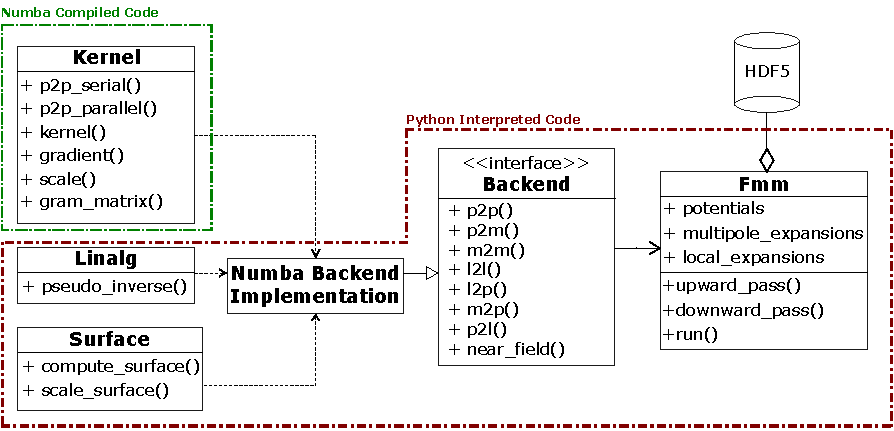
\includegraphics {figures/software.pdf}}
	\caption{Simplified UML model of all PyExaFMM components. Trees and operators are precomputed and stored in the HDF5 database. Except for the `Fmm' object which acts as the user interface, all other components are modules consisting of simple functions.}
	\label{fig:design}
\end{figure*}

\begin{table}
	\centering
	\caption{Effect of compression rank $k$, with multipole and local expansions of order $p=5$, corresponding to $n=98$ quadrature points, for FMM problem with 100,000 randomly distributed points, and a maximum of 150 points per leaf. Point coordinates and charge densities are chosen in the interval [0, 1). Runtimes calculated seven times for statistics, peak memory consumption and relative error reported to 3 significant figures.}
	\begin{tabular}{ |P{10pt}|P{45pt}|P{47pt}|P{47pt}|}
		\hline
		$k$ & Runtime & Peak Memory & Relative Error\\
		\hline
		10 & $6.89 \pm 0.11$s &   663 MB & 1.51e-4\\
		20 & $6.89 \pm 0. 09$s &  667 MB & 2.24e-5\\
		30 &  $6.93 \pm 0. 11$s&  672 MB & 1.15e-5\\
		40 &  $6.95 \pm 0. 09$s &  676 MB & 3.67e-6\\
		98 &  $15.44 \pm 0. 55$s &  685 MB & 2.43e-6\\
		\hline
	\end{tabular}
	\label{tab:compression}
 \end{table}

\section{PERFORMANCE}

Table (\ref{tab:performance}) demonstrates how we achieve similar accuracies in single precision to ExaFMM-T as a function of expansion order as well as the differences in runtime and memory consumption of the two softwares.

\section{CONCLUSION}

We've shown that despite being possible, limitations remain on the efficacy of Python with Numba for HPC. Numba constrains the design of libraries for more complex algorithms, as well as the usage of many Python features. Furthermore, Numba isn't entirely amenable to `drop-in' to existing projects, and has it's own associated learning curve.

Despite achieving runtimes within an order of magnitude of the SOTA, data organization and allocation remains a bottleneck for achieving performance. However, PyExaFMM consists of relatively little source code, and is trivial to deploy on different platforms. Furthermore, as it's written in an interpreted language its development is accessible to non-software specialists. Therefore it remains useful for applications in which runtime is less important, or for rapidly prototyping algorithmic extensions to the FMM.

\section{ACKNOWLEDGMENT}

SK is supported by EPSRC Studentship 2417009.

\bibliography{pyexafmm}
\bibliographystyle{ieeetr}

\begin{IEEEbiography}{Srinath Kailasa}{\,} is a Graduate Student at University College London, currently pursuing a PhD in Computational Mathematics. He received an MPhys in Physics (2017) and an MSc in Scientific Computing (2020) from the University of Durham, and University College London respectively, interspersed with time as a Software Engineer in industry. His research interests are in high-performance and scientific computing. Contact him at srinath.kailasa.18@ucl.ac.uk.
\end{IEEEbiography}

\begin{IEEEbiography}{Timo Betcke}{\,}is Professor of Computational Mathematics at University College London. Is the lead investigator of the Bempp project, an open-source boundary element library. He studied Engineering in Germany as Undergraduate and then completed a PhD in Oxford in Numerical Analysis. From 2005 to 2006 he had various research positions until he became a Lecturer at UCL in 2011. Since 2018 he is a full Professor in the Department of Mathematics at UCL. Contact him at t.betcke@ucl.ac.uk.
\end{IEEEbiography}

\begin{IEEEbiography}{Tingyu Wang}{\,}is a PhD student in Mechanical Engineering at the George Washington University. Contact him at twang66@email.gwu.edu.
\end{IEEEbiography}

\begin{IEEEbiography}{Lorena. A. Barba}{\,}is a Professor of Mechanical and Aerospace Engineering at the George Washington University.  Contact her at labarba@email.gwu.edu.
\end{IEEEbiography}

\end{document}

